% Backward induction step. The value of a state at stage t is computed from the
% already known values at stage t+1. We take the best over the feasible actions.
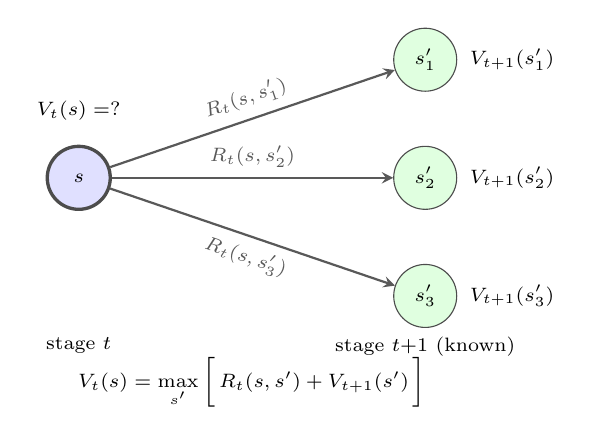
\begin{tikzpicture}[
    x=2.2cm, y=1.0cm,
    state/.style={circle, draw=black!70, minimum size=8mm, inner sep=0pt,
                  font=\scriptsize},
    known/.style={state, fill=green!12},
    cur/.style={state, fill=blue!12, very thick},
    arr/.style={->, >=stealth, thick, black!65},
]
% Stage t (current, unknown) on the left, stage t+1 (known) on the right.
\node[cur] (s) at (0,1.5) {$s$};
\node[known] (a) at (2,3) {$s'_1$};
\node[known] (b) at (2,1.5) {$s'_2$};
\node[known] (c) at (2,0) {$s'_3$};

\node[font=\scriptsize, above] at (0,2.1) {$V_t(s)=?$};
\node[font=\scriptsize, right=1pt] at (a.east) {$V_{t+1}(s'_1)$};
\node[font=\scriptsize, right=1pt] at (b.east) {$V_{t+1}(s'_2)$};
\node[font=\scriptsize, right=1pt] at (c.east) {$V_{t+1}(s'_3)$};

\draw[arr] (s) -- node[above, font=\scriptsize, sloped] {$R_t(s,s'_1)$} (a);
\draw[arr] (s) -- node[above, font=\scriptsize] {$R_t(s,s'_2)$} (b);
\draw[arr] (s) -- node[below, font=\scriptsize, sloped] {$R_t(s,s'_3)$} (c);

\node[font=\scriptsize] at (1,-1.1)
  {$V_t(s)=\max\limits_{s'}\big[\,R_t(s,s')+V_{t+1}(s')\,\big]$};

\node[font=\scriptsize, anchor=north] at (0,-0.4) {stage $t$};
\node[font=\scriptsize, anchor=north] at (2,-0.4) {stage $t{+}1$ (known)};
\end{tikzpicture}
